\documentclass[ThesisDoc]{subfiles}
\begin{document}


% \green{Explicar que son los CSP}
\section{Constraint Satisfaction Problems}
\label{sec:csp}

% \green{Poner una definición no formal}
% \medskip

There are many problems that require positioning or assigning something,
respecting established \emph{restrictions}. \emph{Graph coloring} and
\emph{n-queen} chess problem are classical constraint satisfaction problems (CSPs).

% \medskip
% \green{Poner algunos ejemplos}
% \medskip

The graph coloring problem comes from cartography, where it was needed to color
countries on political maps, in such a way that no country had a land border with
a country of the same color. It was found that \textbf{any} map can be colored
with only four colors.

The n-queen problem is known in chess as \emph{eight queen puzzle}.
Queens in chess can move/attack to/at any square,
that is in a the same row, column or diagonal with the queen.
In the puzzle one needs to place eight (the size of a chess desk)
queens on the desk, so that none of them is threatened by another.
N-queens problems is a generalization of that puzzle, where $n$ queens need
to be placed on a $n \times n$ desk.

Constraint satisfaction problems are found in many areas:
machine vision, natural language processing, theorem proving,
planning and in our problem --- scheduling \cite{MAS}.


\subsection{Formal definition}
%%%%%%%%%%%%%%%%%%%%%%%%%%%%%%%%%%%%%%%%%%%%%%%%%%%%%%%%%%%%%%%%%%%%%%%%%%%%%%%%
\noindent
Formally speaking, a CSP is defined by its \emph{variables} $V$ with the
corresponding \emph{domains} and the \emph{constraints} $\{\xi\}$
over values assignation \cite{MAS}.

\begin{align*}
  V                &= \{v_i\}_{i=1}^N
& \{{\dot v}^i_j\} &= \domain(v_i)
& \xi              &: \{{\dot v}^i_\ast\}_{i=1}^N \mapsto [0,1]
\end{align*}


A variable defines a ``slot'' that can hold a value from the corresponding domain.
A solution to CSP is an assignation of the values ${\dot v}^i_\ast$
to the variables $V$, such that all the restriction hold.
\begin{equation}
  {\dot V} = \{{\dot v}^i_\ast\}_{i=1}^N \text{is a solution}
   \iff \forall \xi \in \{\xi\} \Rightarrow \xi({\dot V}) = 1
\end{equation}

The constraints above are defined in the most generalized form,
over the entire solution. There is a particular case, that is found in many problems
--- \emph{binary constraints}, imposed on \emph{pairs} of values:
$$\xi_2 : \left< {\dot v}^i_\ast, {\dot v}^j_\ast \right> \mapsto \{0,1\}$$

If all constrains are binary, than the satisfaction condition is
$$\forall \xi_2     \in \{\xi\},~
  \forall v_i, v_j  \in V | v_i \not= v_j
~ \Rightarrow ~ \xi_2(v_i, v_j) = 1
$$

\medskip

In the graph coloring problem, the variables are the \emph{colors to be assigned}
for each graph node $\{n_i\}_{i=1}^N$. In this case, all the variables have
the same domain values: four colors, for example \textit{Red}, \textit{Green},
\textit{Blue} and \textit{Yellow}. The constraint is binary and depends on graph
structure:
$$ \xi_2(x,y)= \begin{cases}
  0 & \mbox{if } \exists \text{~edge~} x \leftrightarrow y
                ~\land \text{~color~} x = \text{color~} y \\
  1 & \text{otherwise}
\end{cases}
$$

% For the n-queens problem, there are two ways of representing the variables.One
% can see queens' positions as a single variable --- pairs $\left< x,y \right>$.
% But it's better to handle them separately, as it would be shown in \ref{TODO}.
% In this case each queen would have two variables:
% horizontal and vertical positions $x$ and $y$.

For the n-queens problem, the variables are queens' positions ---
pairs $\left< x,y \right>$, where $x$ is queen's horizontal position and
$y$ is the vertical one. The restrictions can be gathered within a single
constraint function:
$$\xi_2(\left<x_1,y_1\right>, \left<x_2,y_2\right>) =
    \begin{cases}
      0 & \mbox{if } \begin{cases}
                        &      x_1 = x_2  \lor y_1 = y_2 \\
                        \lor~& x_1 = y_2 \land x_2 = y_1 \\
                        \lor~& |x_1-y_1| = |x_2-y_2|
                     \end{cases} \\
     1 & \text{otherwise}
    \end{cases}
$$


  In our \emph{university classes scheduling} problem (UCSP) the variables
are personal schedules, called \emph{timetables} in this thesis,
for each \emph{participant}: professor and group/student.
  A timetable consists of the day-time slots, where classes can be put.
  A \emph{class} is formed for teaching a group a specific \emph{subject},
connecting the participants (of each kind) and establishing a classroom and
the beginning--end \emph{time}.
  Problem \emph{constraints} can be divided into:
\begin{enumerate}
  \item \underline{Class constraints}: a class should be a productive event, so
    a professor should be able to \emph{teach} the class, the classroom should
    have the \emph{capacity} to hold all the students and be properly \emph{equipped},
    and the group should be \emph{enrolled} to class subject
    (further called \emph{discipline}).
  \item \underline{Time constraints}: no participant can have two classes
    at the same time (or intersecting in time), as mentioned before.
  \item \underline{Strong restrictions}: the restrictions, put on a participant, that
    \emph{must} be respected. May include working hours, fixed lunch recess time,
    and any other institution or person specific \emph{obligations}.
  % \item \red{\underline{Weak restrictions} (MOVE)}: the restrictions, that \emph{should} be respected,
  %   but are not critical to the solution. Compliance with these restrictions
  %   raises \emph{solution quality}, but it is assumed that the all of them
  %   cannot be fully met for all the participants --- they are intended to
  %   represent personal \emph{preferences}.
\end{enumerate}

\bigskip

%%%%%%%%%%%%%%%%%%%%%%%%%%%%%%%%%%%%%%%%%%%%%%%%%%%%%%%%%%%%%%%%%%%%%%%%%%%%%%%%
  Until now we were speaking about restrictions satisfaction, but the problem can
be extended to an \emph{optimization} one by defining an
\emph{objective function} over the values configurations.

  Unlike the restrictions (that yield boolean result), the objective functions
should have continuous codomains:
$$\tilde\xi : \{{\dot v}^i_\ast\}_{i=1}^N \mapsto \Re$$
  In order to facilitate the calculations and erase the internal differences of
the objectives, it's often required that the functions must be normalized:
the co-domains are restricted to $[-1,1]$ or $[0,1]$ intervals.

  For example, in case of our UCSP,
one can add \underline{personal preferences} or some institution criteria as
optimization parameters.
  Compliance with the preferences raises \emph{solution quality},
but it is assumed that the all of them cannot be fully met for all the
participants, because \emph{personal} preferences are often
contradictory for different persons.

\subsection{Solution Methods}
%%%%%%%%%%%%%%%%%%%%%%%%%%%%%%%%%%%%%%%%%%%%%%%%%%%%%%%%%%%%%%%%%%%%%%%%%%%%%%%%
% \green{Explicar por qué son importantes computacionalmente}\\
% \medskip

% \noindent
  Solving these problems usually presents difficulties due to the amount of
possible combinations to consider for a solution. Let's have a look at
some university schedule.
  For example, six working days in a week and twelve time slots every day
(every hour from 8:00 to 20:00), would yield $6 \times 12 = 72$ options
to place each class.
  Given that each group needs, for example, five different disciplines to be assigned,
there would be $\multibinom{72}{5} = \num[group-separator={,}]{18474840}$
possible classes assignments for each group,
even without considering professors and classrooms.

% \bigskip
% %%%%%%%%%%%%%%%%%%%%%%%%%%%%%%%%%%%%%%%%%%%%%%%%%%%%%%%%%%%%%%%%%%%%%%%%%%%%%%%%
% \green{Explicar formas de resolver los CSP} \todo
\medskip
\noindent

  The researchers have been looking for means of solving such
problems within reasonable time.
  During the last years different algorithms and techniques where developed,
such as
\emph{dynamic constraint satisfaction based on extension particle swarm
      optimization algorithm} \cite{CSPswarm},
\emph{dynamic state bounding} \cite{CSPdynStateBound},
\emph{conflict-vector detection} \cite{CSPtimetable},
\emph{neural networks} \cite{CSPneuro},
\emph{ant colony optimization} \cite{CSPcunningACO, CSPlimmemACO},
\emph{selective hyper-heuristics} \cite{CSPhypHeur}
and \emph{agents} \cite{CSPagent2013, CSPagent2014, DCSPagent1998}.

\medskip

Those methods do not seek for the optimal solutions, focusing instead on
``rather good'' ones, that can be obtained within reasonable time using admissible
computing resources.

\bigskip

% \todo \red{: write something about one of the techniques}



\subsection{\red{Distributed problems}}
%%%%%%%%%%%%%%%%%%%%%%%%%%%%%%%%%%%%%%%%%%%%%%%%%%%%%%%%%%%%%%%%%%%%%%%%%%%%%%%%
Agents approach allows solving CSPs in a distributed manner, also distributing
the problem knowledge and constraints
\cite{DCSPagent1998, DCSP2013, CSPagent2014, MAS, MAS-Survey}.

\begin{displayquote}[\cite{MAS-Survey}] % \cite[p.~2]{MAS-Survey}
  For example, a constraint satisfaction problem can often be
  decomposed into several not entirely independent
  subproblems that can be solved on different processors. $\dots$
  MAS (Multiagent System) allows the sub-problems of a constraint satisfaction
  problem to be subcontracted to different problem solving agents with their own
  interests and goals.
\end{displayquote}

\noindent
Such problems are \emph{Distributed Constraints Satisfaction Problems} (DCSPs).
\begin{displayquote}[\cite{MAS}] % \cite[p.~4]{MAS}
  In a distributed CSP, each variable is owned by a different agent. The goal is
  still to find a global variable assignment that meets the constraints, but each agent
  decides on the value of his own variable with relative autonomy. While he does
  not have a global view, each agent can communicate with his neighbors in the
  constraint graph.
\end{displayquote}

  The constrains are distributed alongside the variables: an agent knows only the
constrains over the variable it owns. A DCSP can also have objective functions for
optimization.

  The UCSP fits perfectly into a the DCSP class: timetable variables,
strong restrictions and personal preferences are determined by agent's creator
and his interests. The class and time constraints apply to all the agents and
represent common behavior base.

  The original UCSP is decomposed in a set of sub-problems, one for each participant.
A sub-problem consist in resolving constraints over a \emph{timetable} variable.
Some sub-problems are interdependent through \emph{classes connections}. In this
case, the timetable configurations of the connected agents must be negotiated
until consensus is reached. If some agents cannot reach it, they could change the
class, searching for another participant.

  The solution to the original problem is a list of participants with the corresponding
timetables. The last ones are gathered, after all sub-problems have been resolved.

% At the figure \ref{fig:ScheduleSpace} the university schedule is
% shown as a 3-dimentional table; horizontal rectangles represent individual
% schedules for the corresponding participants.

% \begin{figure}
%   
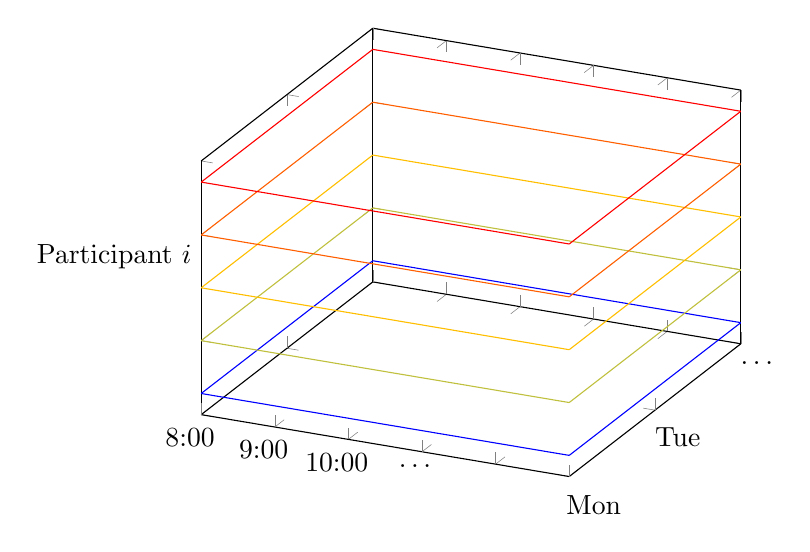
\begin{tikzpicture}

\begin{axis}[
  xlabel=, % Time,
  xticklabels={, 8:00, 9:00, 10:00, $\dots$},
  ylabel=, %Day,
  yticklabels={, Mon, Tue, $\dots$},
  zlabel=, %Participant,
  zticklabels = {, , ,Participant $i$}
  ]

  \foreach \i in {1,...,5}
     \addplot3[surf] coordinates { (0,0,\i) (1,0,\i) (1,1,\i) (0,1,\i) (0,0,\i)  };

  % \addplot3[surf] coordinates { (0,0,0) (1,0,0) (1,1,0) (0,1,0) (0,0,0)  };
  % \addplot3[surf] coordinates { (0,0,1) (1,0,1) (1,1,1) (0,1,1) (0,0,1)  };

\end{axis}


\end{tikzpicture}

%   \caption{Distributed university schedule.}
%   \label{fig:ScheduleSpace}
% \end{figure}


\end{document}
